%%=============================================================================
%% Methodologie
%%=============================================================================

\chapter{\IfLanguageName{dutch}{Methodologie}{Methodology}}
\label{ch:methodologie}

%% TODO: Hoe ben je te werk gegaan? Verdeel je onderzoek in grote fasen, en
%% licht in elke fase toe welke stappen je gevolgd hebt. Verantwoord waarom je
%% op deze manier te werk gegaan bent. Je moet kunnen aantonen dat je de best
%% mogelijke manier toegepast hebt om een antwoord te vinden op de
%% onderzoeksvraag.
Aucxis werkt momenteel hoofdzakelijk met ‘.NET’ projecten. Als IDE wordt er Visual Studio gebruikt. Als versiebeheer gebruiken ze hiervoor TFVC. Dit was een voor een lange tijd een goede oplossing. De testen die werden uitgevoerd waren vooral functionele testen. Dit is niet ideaal. Er wordt op moment van implementatie bij klanten veel fouten en bugs vastgesteld waardoor er enerzijds veel frustratie ontstaat bij de mensen die het uitrollen bij een klant. Anderzijds wordt er veel tijd en geld verloren met het over en weer verplaatsen tussen klant en bedrijf. Aucxis heeft recent een keuze gemaakt om meer te investeren in kwaliteit. Aangezien Aucxis al een verwent gebruiker van Microsoft is, was de keuze voor Azure DeVops niet moeilijk. Ook heeft dit minder impact op hun huidige werkwijze.

Zoals eerder aangehaald worden er vooral functionele testen uitgevoerd. Met de stap naar kwalitatievere oplossingen is er ook nood voor meerdere soorten testen. Het ideale zou zijn dat er naast functionele testen ook in een gecontroleerde omgeving, die een situatie bij de klant in kwestie nabootst, getest kan worden. Daarna zou het programma bij een test omgeving van de klant uitgerold worden om daar te worden getest. In een finale stap, zou het programma dan in productie worden uitgerold. Dit alles zou zo geautomatiseerd mogelijk moeten verlopen.

Azure DeVops lijkt hier het meest geschikt voor om deze functionaliteit te verkrijgen. Daarom de vraag om toch het aanbod van Azure met de andere Cloud platform aanbieders te vergelijken en het beste alternatief te selecteren. Om dit te bereiken is er in dit onderzoek begonnen met kort de verschillende Cloud platformen hun aanbod naast elkaar te leggen.

\section{Vergelijking}
\subsection{Azure DeVops}
Microsoft Azure is gelanceerd in 2010 en bevat een hele serie producten. Azure biedt vooral producten aan in de categorieën Software as a Service (SaaS), Infrastructure as a Service (Iaas) \& Platform as a Service (PaaS). Azure heeft een aantal zeer goede producten voor virtualisatie. Zo Biedt Azure een enorm aanbod aan verschillende soorten machines aan voor verschillende doeleindes. Ook hun virtuele netwerkmogelijkheden zijn enorm. Dit alles is mooi geordend en zeer gemakkelijk in gebruik. De Azure datacenters zijn over heel de wereld verspreid. Deze zijn altijd het nieuwste van het nieuwste en zijn zeer goed verbonden onderling en met de buitenwereld. Omdat Azure van Microsoft is, is Azure ook perfect te integreren met bestaan gebruikers accounts in domeinen. Dit geeft de gebruiker volledige controle over wie wat kan gebruiken en zien. Azure biedt ook een aantal services aan. Daarvan is Cloud gebaseerde Active Directory er een van. Ook bieden ze een volledig aanbod aan services aan om een CI/CD pijpleiding te realiseren.

Azure DeVops was vroeger bekend als Visual Studio Team System (VSTS) of Team Foundation Server (TFS). Het is een versie beheer, rapportering, vereisten beheer, project beheer, automatisch compileer, test en uitrol beheer tool gemaakt door Microsoft. De tool maakt gebruik van Team Foundation Version Control (TFVC) of Git. De tool is gemaakt om de volledige levenscyclus van een programma te controleren en beheren. Ook biedt de tool de mogelijkheid aan programmeerteams om in een DeVops sfeer samen te werken. Het mooie aan deze tool is dat het bijna in iedere Integrated Development Environment (IDE) te integreren is.

Het is mogelijk om deze tool zowel lokaal als in de Cloud te implementeren. Microsoft heeft deze tool toegevoegd aan hun Azure aanbod onder Azure DeVops. Microsoft heeft de verschillende componenten van deze tool opgesplitst op het platform. Dit maakt het mogelijk dat de gebruiker niet alle componenten tegelijk hoeft te gebruiken of te implementeren. De gebruiker kan zo naar hun voorkeur functie kiezen.

Azure DeVops kan gebruikmaken van twee soorten versie controle in een project. Het kan gebruikmaken van de door Microsoft speciaal ontwikkelde versie beheer framework TFVC voor Azure DeVops of het wereld befaamde Git. 

TFVC ondersteund twee manieren van werken, met een centraal systeem of lokaal met check-out/ check-in op de computer van de programmeur. Bij het gebruik van een centraal systeem worden files die door een andere programmeur gebruikt worden als ‘alleen lezen’ bestempeld. Dit kan leiden tot problemen als andere programmeurs deze files nodig hebben voor bepaalde zaken. Dit heeft Microsoft proberen oplossen door het mogelijk te maken om volledig lokaal te werken. De programmeur kan dan alle files aanpassen waar nodig. Eventuele problemen met verschillende files moeten dan worden opgelost bij check-in. Dit maakt het mogelijk dat er veel minder conflicten ontstaan. Een ander voordeel is dat de gebruiker de mogelijkheid heeft om met TFVC, regels te configureren die bij check-in worden uitgevoerd.

Git is een veel gebruikt versie beheersysteem. Bijna alle IDE’s bieden ondersteuning aan voor dit systeem. Het werkt gelijkaardig zoals TFVC. Alleen kan de gebruiker met Git geen regels configureren die worden uitgevoerd bij check-in. Git is wel volledig compatibel met Azure DeVops. Zo kan er rechtstreeks met Git op Azure DeVops gepubliceerd worden. Dit alles zorgt ervoor dat gebruikers door gebruik van Git, met bijna iedere IDE of programmeertaal, Azure Devops kan gebruiken. 

Een ander voordeel van Azure DeVops is de uitgebreide rapportering ingebouwd in de tool. Deze maakt het mogelijk om uitgebreide verslagen te genereren van de uitgevoerde testen, een uitgevoerde check-in, compilatie problemen, enz. Ook staat het de gebruiker toe om gepaste meldingen te versturen of automatisatie te configureren om bepaalde problemen op te lossen. Daarnaast heeft Azure Devops ook een ingebouwde tool om planningen voor projecten bij te houden.

Azure Boards is letterlijk een volledige implementatie rechtstreeks in Azure DeVops van een scrum bord. Zo kan de gebruiker bij het opleveren van een uitgevoerde taak automatisch de compilatie pijpleiding laten starten. Ook is het volledig geïntegreerd met GitHub waardoor de gebruiker geen extra kosten moet maken om een Azure Repository aan te maken. Ook bestaat de mogelijkheid om Azure boards naadloos te laten samenwerken met de populairste chat applicaties voor ontwikkelaars, zoals Slack.

In Azure DeVops als een gebruiker een CI pijpleiding wil configureren, kan de gebruiker dat simpel via de web interface doen of met de Azure powershell add-on. Azure DeVops gebruikt zoals eerder vermeld, twee soorten versie beheer tools. Om met Git een pijpleiding te bouwen selecteert de gebruikt simpel weg als bron een git repository. Daarna kan de gebruiker kiezen uit een hele serie voor gemaakte motoren voor het compileren van de code. Ook door gebruik te maken van een marktplaats kunnen er zelfs volledig aangepaste motoren gebruikt worden. Hierna wordt de gebruiker gevraagd om een azure-pipelines.yml aan te maken in de broncode waarin dan de configuratie geschreven wordt voor de uit te voeren compilatie. De gebruiker kan dan nog stappen toevoegen voor testen uit te voeren. Azure DeVops heeft de mogelijkheid om op verschillende manieren de software uit te rollen. Gaande van in de Cloud naar specifieke lokale omgevingen enz.

Azure Devops prijzen worden beschreven in figuur~\ref{fig:A_DO_Money}.

\begin{figure}[!htbp]
    \centering
    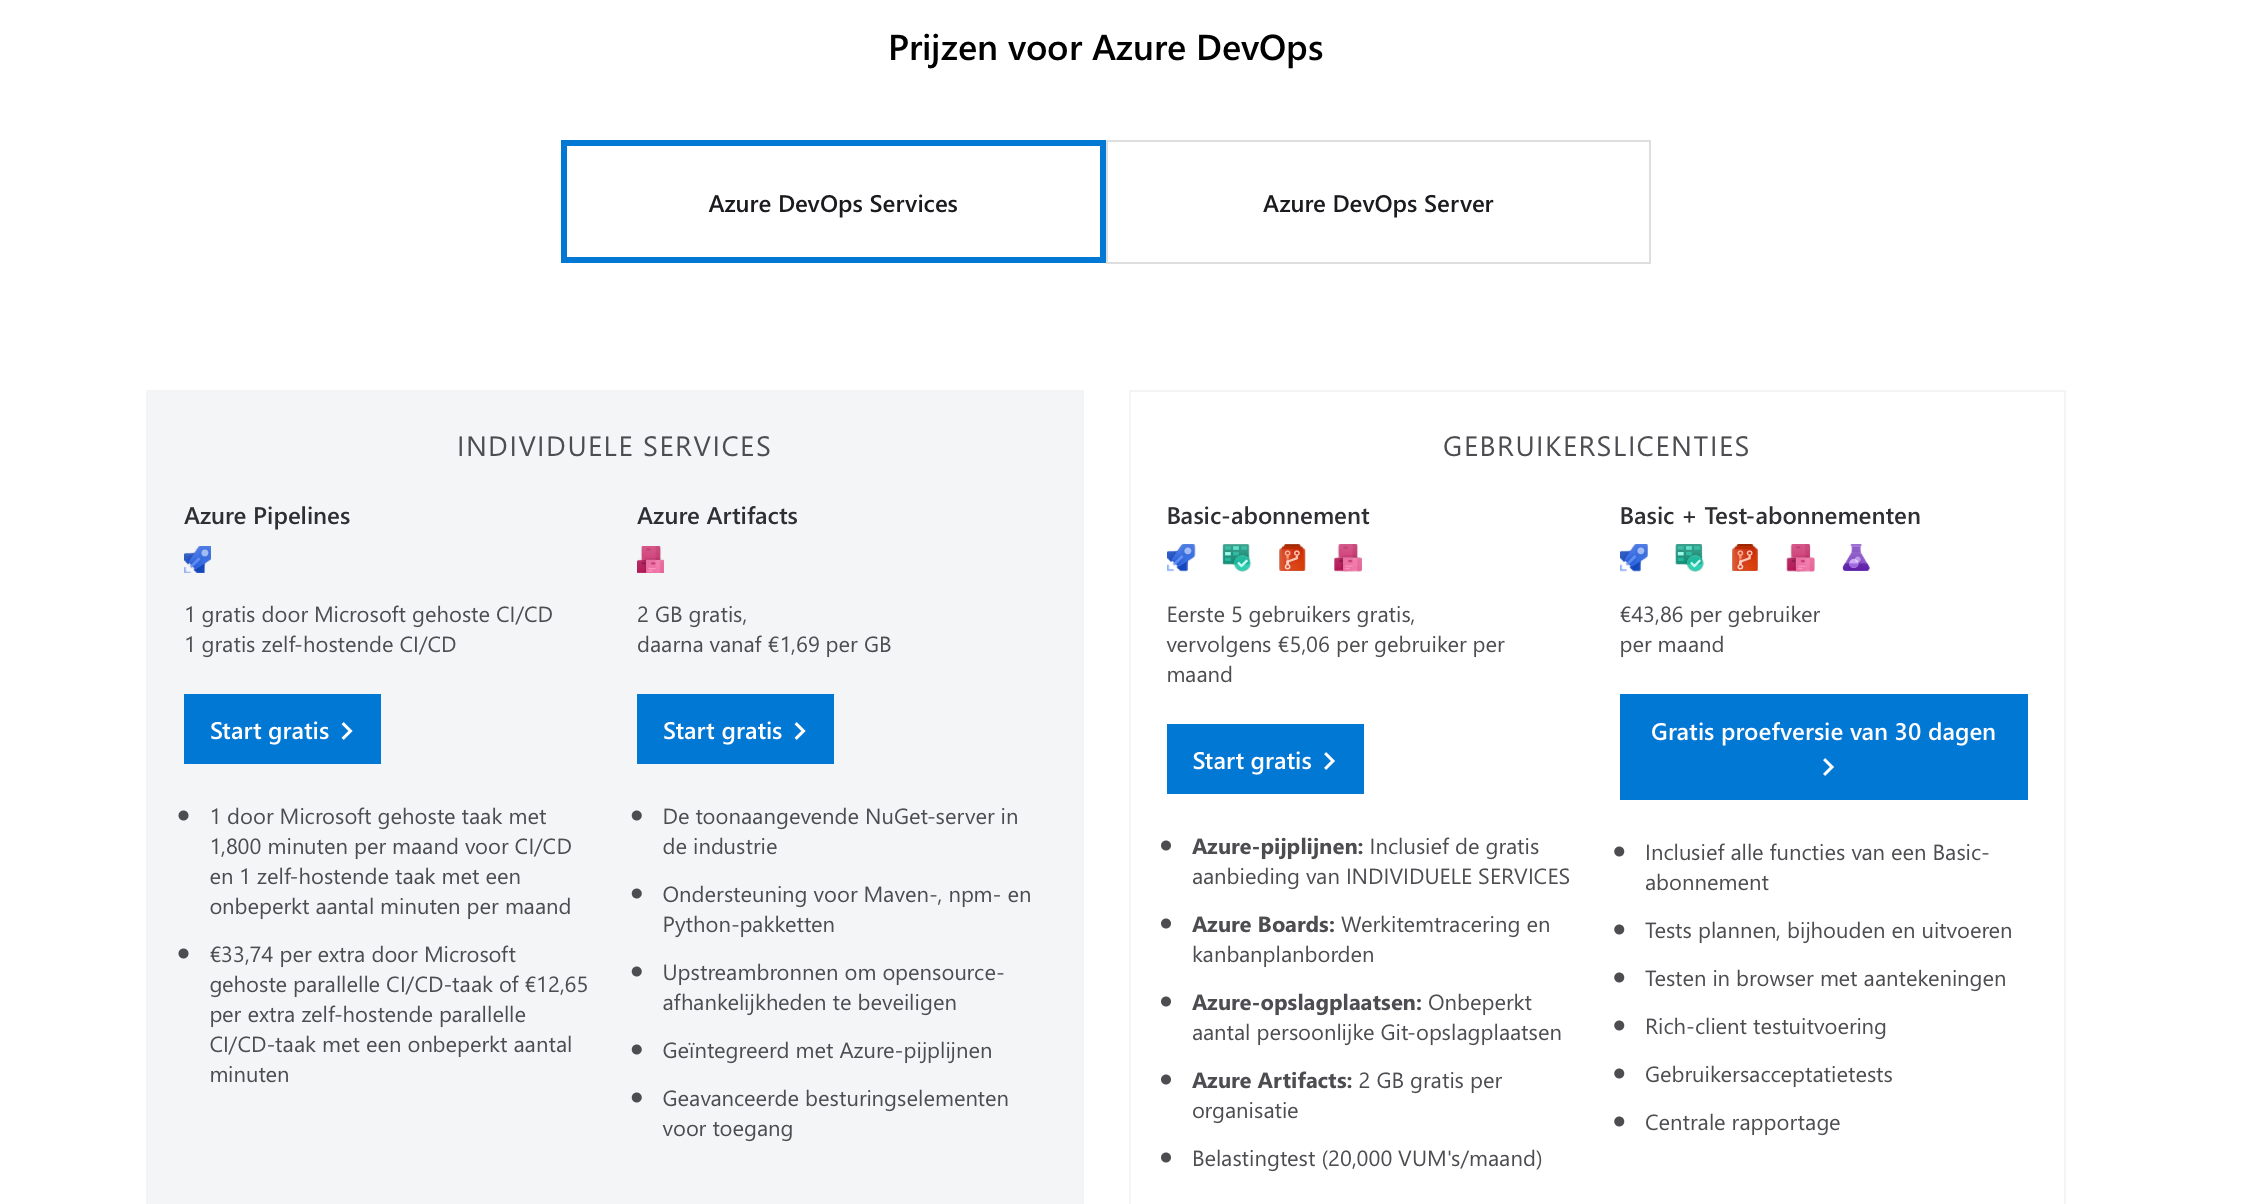
\includegraphics[width=\linewidth]{/Users/kenzie/Documents/HoGent/Bachelorproef/Images/Azure_DO_money.png}
    \caption{Figuur van \href{https://azure.microsoft.com/nl-nl/pricing/details/devops/azure-devops-services/}{Azure DeVops website}. Figuur toont de prijzen voor Azure DeVops op een beknopte manier.}
    \label{fig:A_DO_Money}
\end{figure}

Azure DeVops is in dit onderzoek het vertrekt punt voor de vergelijkingen. Dit omdat het perfect met de huidige werkwijze van Aucxis integreert en omdat zij reeds Microsoft partner zijn. In alle vergelijkingen zal gekeken worden of Git gebruikt kan worden omdat dit het een stuk gemakkelijker maakt voor de vergelijkingen. Aucxis ontwikkelt veel applicaties in .NET Core en daarom moet er ook gekeken worden of de alternatieve hiervoor compatible zijn. Azure DeVops is dus het zeer capabele vertrek punt voor de vergelijkingen met de andere Cloud platform aanbieders.
\subsection{Google Cloud}
Google Cloud Platform (GCP) is gelanceerd in April 2008. Het draaide des tijds in dezelfde datacenters als ‘google search’, ‘youtube’ en ‘gmail’. Het was slechts in 2011 dat GCP beschikbaar was voor het brede publiek. GCP is een onderdeel van de Google Cloud. Google Cloud biedt een enorme serie van producten aan waarvan GCP maar een klein onderdeel is. GCP specifiek, biedt ‘infrastructure as a service’ (IaaS), ‘platform as a service’ (PaaS) en ‘serverless computing’ aan. 

Omdat het doel van dit onderzoek specifiek de support voor CI/CD pijpleidingen vergelijken is, bekijken we een specifiek onderdeel van GCP. De ‘Cloud Developper Tools’. Onder deze categorie vallen er een aantal zeer interessante tools. Hier vindt men onder andere ‘Cloud Build’, ‘Cloud-SDK’, ‘Tools voor Powershell’, ‘Tools voor Visual Studio’, enz.

Cloud Build is Google zijn antwoord op een volledige geautomatiseerde CI/CD pijpleiding. Het is dan ook volledig mede met de moderne vereisten. Met Google Cloud Build (GCB) is een organisatie instaat om snel en gemakkelijk een volledige pijpleiding te configureren. Het gelijkt dan ook op Azure DeVops.

GCB werkt hoofdzakelijk met Git en GitHub om een pijpleiding te bouwen. Google heeft ook zijn eigen ‘Cloud repository service’ die naadloos integreert met GCB, maar deze is helaas betalend. Daarom is het gebruik van Git met GitHub een beter en goedkoper alternatief. Aangezien deze ook perfect integreren met GCB en omdat Git wijdverspreid en simpel in gebruik is. Een organisatie kan dan configureren op GCB dat bij het moment van een code update op GitHub, automatisch een compileer pijpleiding wordt gestart. Om GCB te laten weten wat er specifiek moet uitgevoerd worden, moet er op de GitHub repository een YML-file voorzien worden waarin regels gedefinieerd moeten worden. Dit maakt het gemakkelijk om snel aanpassingen te maken.

De pijpleiding op GCB werkt op basis van Docker images. Deze worden in de cloudbuild.yml gedefinieerd. Ook wordt er per Docker container gedefinieerd wat er moet uitgevoerd worden in de vorm van commando’s, script, enz. Dit maakt het mogelijk dat iedere stap in het CI gedeelte van de pijpleiding volledig aangepast kan worden naar de noden van de organisatie. Zo kan de organisatie beslissen om voor gemaakte containers te gebruiken van de ‘DockerHub’ pagina. Ook kan de organisatie zelf container maken met aangepaste scripts om bijvoorbeeld in lokale omgevingen testen uit te voeren. GCB kan dus in een hybride opstelling geïmplementeerd worden. Wat ook de bedoeling zou zijn aangezien dit een use case van Aucxis is. Daarnaast biedt GCB ook de mogelijkheid om de gecompileerde code rechtstreeks vanuit Google Cloud beschikbaar te maken voor verdere verdeling.

Met behulp van deze containers kunnen dan functionele testen uitgevoerd worden op de gecompileerde code. Het programma kan dan op basis van de uitkomst van deze uitgevoerde taak, naar de volgende stap zijn wachtrij worden geplaatst. Hier kan dan de volgende taak starten. GCB genereert rapporten en statistieken van de uitgevoerde taken zodanig dat de gebruiker van het platform inzicht kan krijgen in de uitgevoerde taken.

De compilatie en uitvoer-tijden van GCB zijn zeer goed aangezien het platform automatisch schaalt naarmate er meer rekwesten tegelijk verstuurd worden. Dit maakt mogelijk dat verschillende programmeurs tegelijk aan hetzelfde project werken of aan meerdere projecten tegelijk. Ook biedt GCB de mogelijkheid om redundantie te voorzien. GCB maakt het mogelijk om naar andere Cloudplatformen uit te rollen of zelfs om de werklast te verdelen over verschillende Cloud platformen. Dit is mogelijk door gebruik te maken van Tekton. Tekton is een open-source framework voor Kubernetes. Dit maakt het mogelijk dat een organisatie over verschillende Cloud platformen heen kan werken. Kubernetes is een clustering hypervisor voor Docker containers. Tekton zou een goede oplossing kunnen zijn voor CI/CD pijpleidingen in de Cloud maar valt hier buiten beschouwen vermits het doel de verschillende aanbiedingen van de Cloud platformen vergelijken is.

De prijzen in Google Cloud worden berekend zoals bij ieder moderne Cloud aanbieder. De gebruiker betaald wat hij verbruikt. De volgende figuur~\ref{fig:GCP_BC_money} moet dienen om een beeld te vormen over wat men kan verwachten te betalen voor het gebruik van GCB. Dit zonder netwerk kosten voor het transfereren van gegevens. Er wordt ook niks in rekening gebracht voor zaken die in een wachtrij staan of pijpleidingen die niet gebruikt worden. De Google Cloud Developper Tools hebben een voordeel dat een groot deel van de tools voor ondersteuning met het platform gratis zijn. Er zijn ook weinig tools van derden nodig om de gewilde functionaliteit te bereiken.

\begin{figure}[!htbp]
    \centering
    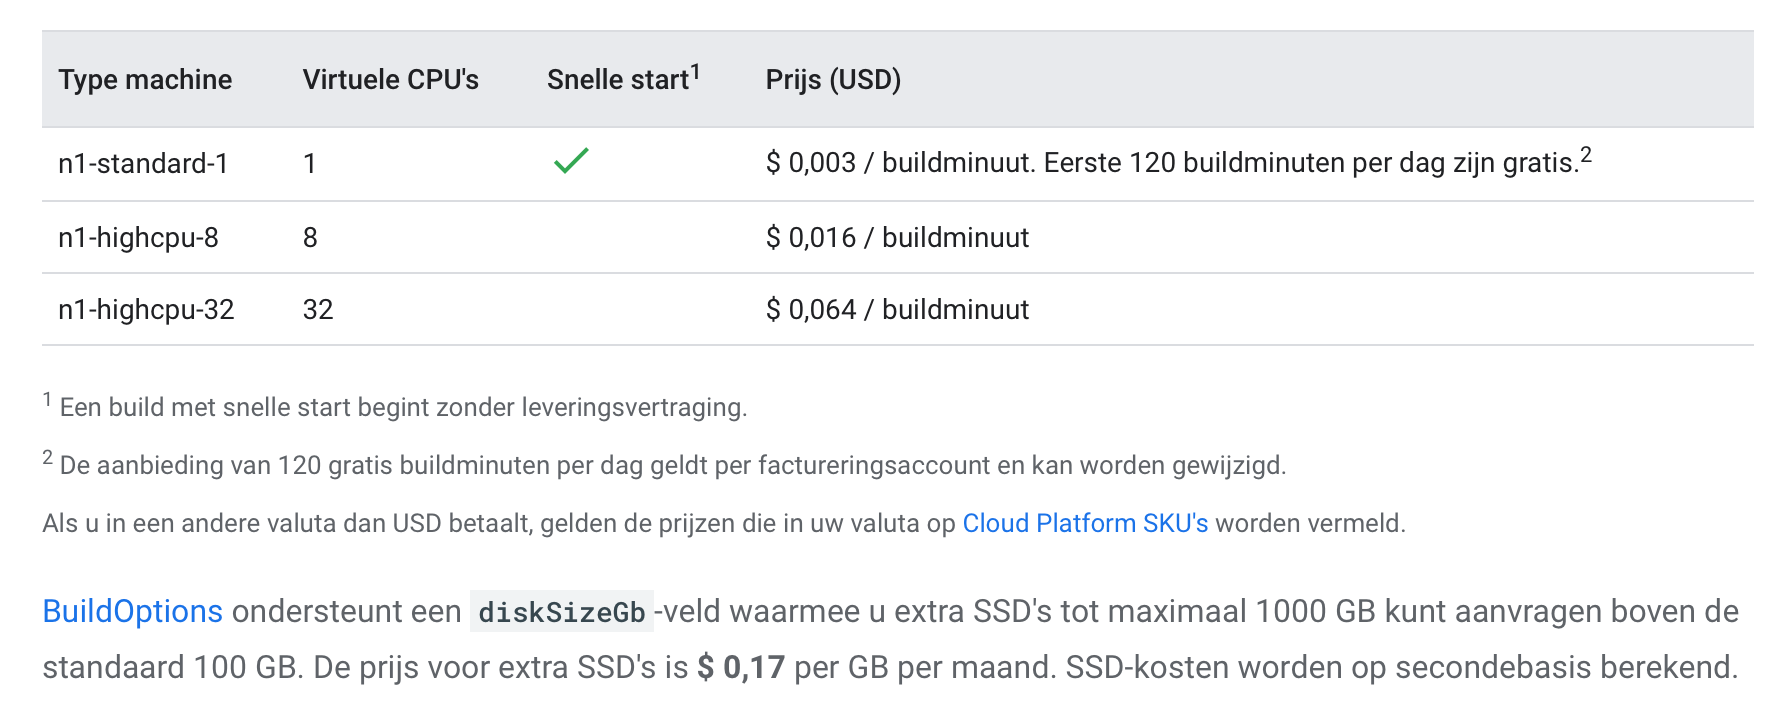
\includegraphics[width=\linewidth]{/Users/kenzie/Documents/HoGent/Bachelorproef/Images/gcp_bc_money.png}
    \caption{Figuur van \href{https://cloud.google.com/cloud-build/pricing}{Google Cloud website}. Figuur toont de prijzen voor Google Cloud Platform op een beknopte manier.}
    \label{fig:GCP_BC_money}
\end{figure}

Met andere woorden is GCB dus een volwaardig alternatief voor Azure DeVops. Er is ondersteuning voor verschillende tools, biedt uitgebreide functionaliteiten aan en bovendien adverteert Google dat het gemakkelijk samenwerkt met andere Cloudplatformen. Het zei door het gebruik van Tekton. Daarnaast is het ook relatief simpel in gebruik door dat GCB gebruikmaakt van Docker containers voor te compileren.

\subsection{Amazon Web Services}
Amazon web services (AWS) is gelanceerd in 2006. Gedurende lange tijd heeft Amazon stukken van hun datacenter verhuurd aan het brede publiek. Tegenwoordig kan een gebruiker op AWS een Cloud computer samenstellen juist zoals een gewone server samengesteld zou worden. Het is maar in recente tijden dat Amazon zich meer beginnen focussen is op services die de gebruiker kan gebruiken. Zo bevat AWS nu meer dan 212 services en producten. Bijvoorbeeld: virtuele computerkracht, netwerking, opslag in de Cloud, databases, statistieken, programma services, uitrol op de Cloud, beheer van bepaalde zaken, programmeertools en tools voor Internet Of Things (IoT). De populairste tegenwoordig zijn Amazon Elastic Compute Cloud (EC2) en Amazon Simple Storage Service (Amazon S3). Deze laatste zijn in feite Cloud computerkracht en opslag voor van alles die volledig schaalbaar zijn en die geen kosten hebben om aan te maken.

Ondanks dit groot aanbod resteert er toch nog altijd de vraag hoe het zit met de huidige prestatie van Amazon datacenters over de hele wereld. Zeker na het lezen van deze paper \autocite{Jackson2010}. Voor dit onderzoek is er ijverig gezocht naar recentere prestatie onderzoeken maar zonder resultaat. Er kan alleen maar afgegaan worden van Amazon zijn website.

Al deze producten en services maken het niet gemakkelijk voor een gebruiker om snel te weten welke producten juist voor hem geschikt zijn. Ook in dit onderzoek is er vastgesteld dat het lastig was om een duidelijk beeld te krijgen wat er allemaal aangeboden wordt. Dat terzijde, heeft Amazon toch een specifiek aanbod om CI/CD pijpleidingen te implementeren op hun Cloud platform. Zo heeft Amazon, AWS CodePipeline. Dit is een service waarbij de gebruiker of organisatie via het web portaal gemakkelijk een CI/CD pijpleiding kan definiëren. Deze is volledig aanpasbaar naar de noden van de gebruiker. AWS CodePipeline gebruikt AWS CodeBuild voor de compilatie en het testen van projecten in CI/CD en AWS CodeDeploy voor de automatische uitrol van projecten.

Zoals alle grote Cloud platformen ondersteund AWS CodePipeline ook het gebruik van Git en GitHub. De gebruiker hoeft dus geen speciale zaken te doen. Amazon heeft ook zijn eigen Cloud repositories voor code in op te slaan. Deze zijn ook gebaseerd op Git. Het zijn eigenlijk privé Git repositories die door Amazon worden aangeboden. Het gebruik verschilt niet tussen GitHub en Amazon zijn privé Git servers. De gebruiker kan gemakkelijk via het web portaal de gewenste Git-projecten toevoegen aan AWS CodePipeline.

AWS CodeBuild is een CI service die code compileert, testen uitvoert en als resultaat uitrolbare software oplevert. AWS CodeBuild is speciaal omdat er geen nood is om zelf de server infrastructuur te configureren voor de compilatie van code. AWS CodeBuild doet dit allemaal voor de gebruiker en schaalt mede naarmate de belasting of het project groter wordt. AWS CodeBuild maakt gebruik van voorverpakte compileer omgevingen maar de gebruiker heeft wel de mogelijkheid om zelf zijn compilatie omgevingen te configureren. Dit maakt mogelijk dat de pijpleiding volledig aan te passen is naar de noden van de gebruiker. Zodat Amazon weet wat voor compilatie omgeving er moet gebouwd worden, moet de gebruiker aan de project folder een BuildSpec.yml toevoegen waarin staat welke compileer motor er gebruikt moet worden met welke files. Dit kan ook gedefinieerd worden in het web portaal zodanig dat de gebruiker niet de hele tijd de broncode moet updaten bij wijzigingen aan de configuratie. Ook heeft AWS CodeBuild een voordeel. Na dat de compilatie en testen geslaagd zijn kan er direct een zip gemaakt worden die dan downloadbaar is van Amazon zijn Cloud opslag. Dit is een voordeel aangezien het bij Google niet duidelijk was of dit mogelijk is op die manier. Google wilt alles verpakken in Docker containers die dan wel beschikbaar zijn. AWS CodeBuild zijn prijzen worden op dezelfde manier berekend als Google Cloud Build. Er wordt betaald per minuut dat er computerkracht gebruikt wordt. Zie de figuur~\ref{fig:AWS_CB_money} en figuur~\ref{fig:AWS_CB_money2}

\begin{figure}[!htbp]
    \centering
    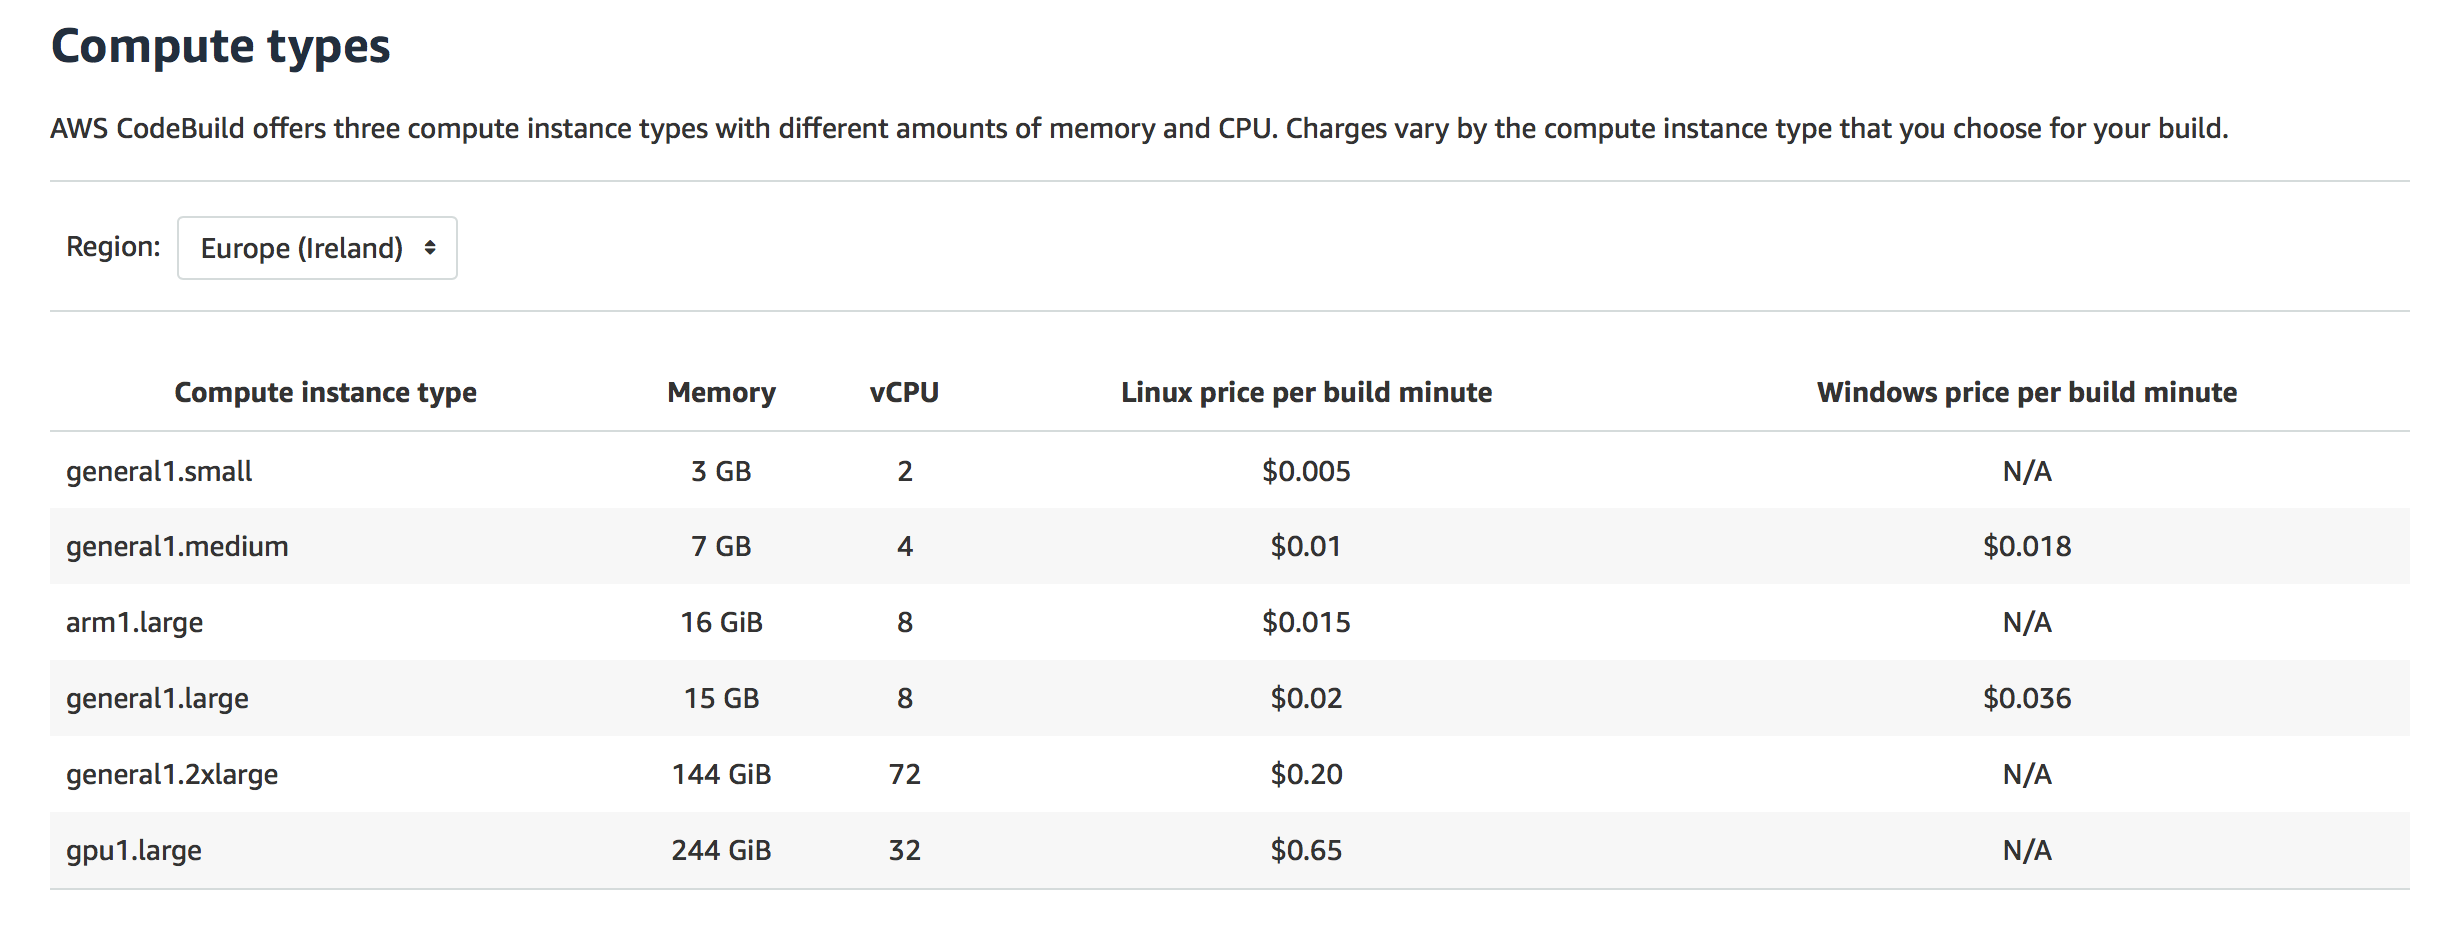
\includegraphics[width=\linewidth]{/Users/kenzie/Documents/HoGent/Bachelorproef/Images/AWS_CB_money.png}
    \caption{Figuur van \href{}{AWS website}. Figuur toont de prijzen van AWS per rekenkracht, OS en verstreken minuut.}
    \label{fig:AWS_CB_money}
\end{figure}
\begin{figure}[!htbp]
    \centering
    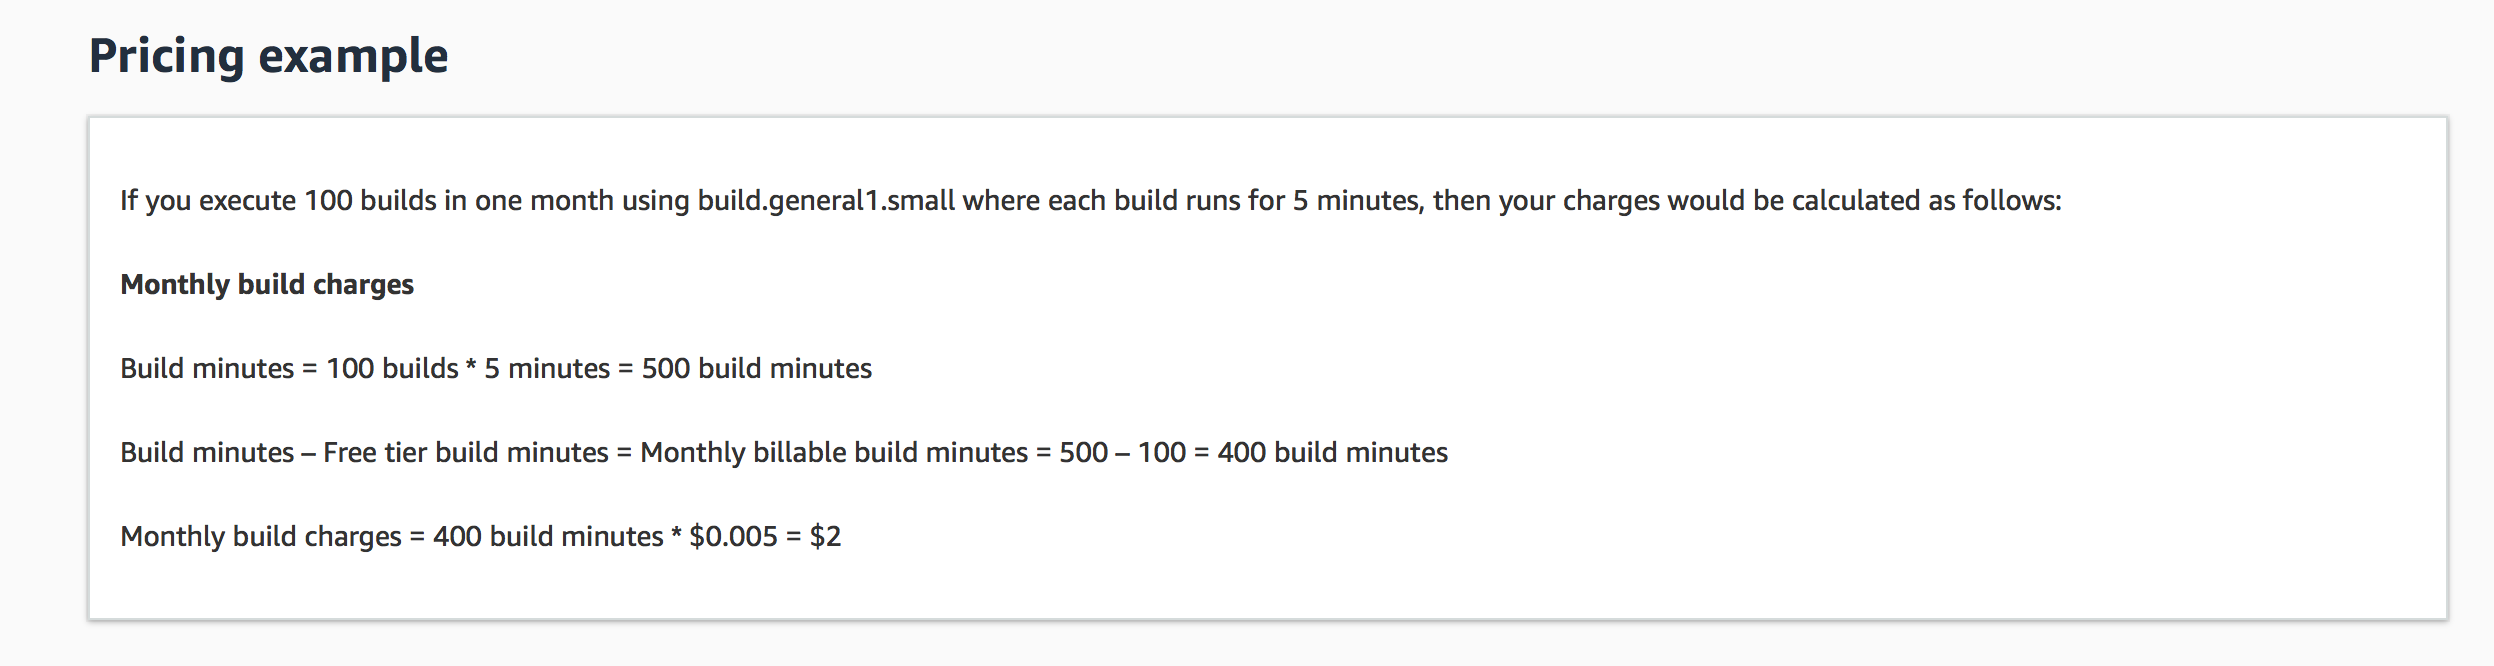
\includegraphics[width=\linewidth]{/Users/kenzie/Documents/HoGent/Bachelorproef/Images/AWS_CB_money2.png}
    \caption{Figuur van \href{}{AWS website}. Figuur toont berekening van prijzen per compileer minuut voor AWS.}
    \label{fig:AWS_CB_money2}
\end{figure}

Een klein detail dat maar zichtbaar was bij het bekijken van de prijzen stelsels. De gebruiker heeft de mogelijkheid om een besturingssysteem (OS) te kiezen bij het aanmaken van een AWS CodeBuild pijpleiding. Dit onderzoek heeft vastgesteld dat een Windows OS wel beschikbaar is maar niet in iedere datacenter locatie. Vaak is die optie ook duurder dan de Linux variant. Dit kan eventueel problemen veroorzaken met Windows specifieke voorbeelden. Ook is het moeilijk om informatie te vinden over hoe de gebruiker nu juist zelf een aangepaste compilatie motor definieert. 

AWS CodeDeploy is het CD gedeelte van de AWS CodePipeline. Het is volledige te beheren en aanpasbaar naar de noden van de gebruiker. Zo is het mogelijk om rechtstreeks vanuit de pijpleiding uit te rollen naar eender welke Amazon Cloud service of naar lokale omgevingen. Aangezien het mogelijk is om een zip met de software in te downloaden is het ook gemakkelijk te integreren met bestaande uitrol tools of werkwijzen. Deze feature is ook niet gratis. Volgende figuur~\ref{fig:AWS_CD_money} toont dit aan. Amazon rekent per update van een instantie een prijs aan. Daarbovenop moet er ook nog betaald worden voor de verbruikte opslag.

\begin{figure}[!htbp]
    \centering
    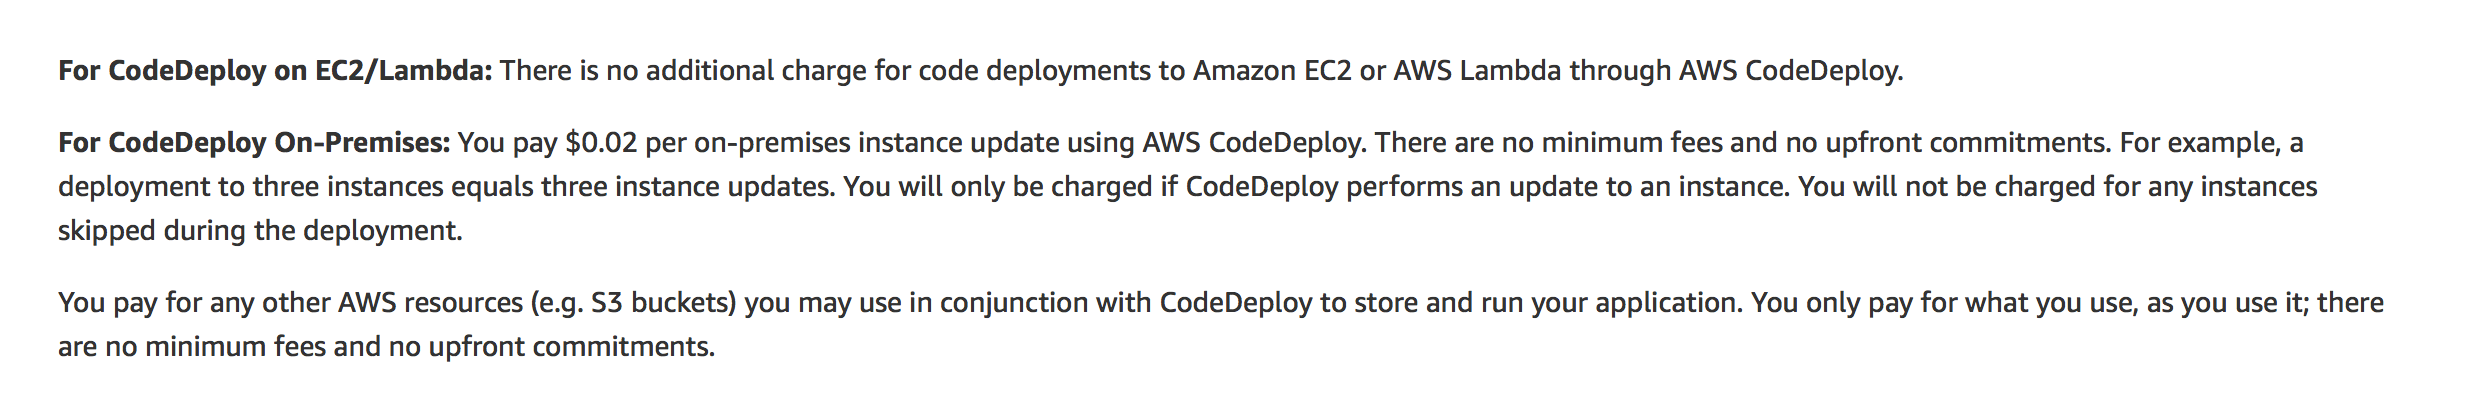
\includegraphics[width=\linewidth]{/Users/kenzie/Documents/HoGent/Bachelorproef/Images/AWS_CD_money.png}
    \caption{Figuur van \href{}{AWS website}. Figuur toont prijs voor opslag op AWS.}
    \label{fig:AWS_CD_money}
\end{figure}

Naast een hele serie ontwikkeltools heeft Amazon ook tools toegevoegd om gedetailleerde rapporten en analyses te genereren van de uitgevoerde taken op AWS CodePipeline. Dit geeft juist zoals Google, de gebruiker goede inzichten in wat er juist allemaal gebeurt en verkeerd loopt. Ook kan de gebruiker op basis van foutmeldingen of status rapporten bepaalde acties instellen en laten uitvoeren.

Het zou mogelijk zijn om met AWS de gewilde functionaliteit de realiseren. Het zal wel zeer arbeid intensief zijn aangezien informatie over zelf een compilatie motor maken moeilijk te vinden is. Ook is het een stuk duurder. Dit onderzoek heeft ook vastgesteld dat Amazon een hele reeks van producten heeft waardoor het soms moeilijk is om door het bos de bomen te zien. Ook de prestatie van het platform blijft een vraagteken door de paper \autocite{Jackson2010}.

\subsection{IBM Cloud}
IBM Cloud is mogelijk een van de oudere Cloud platformen. Voor dat de term Cloud veel gebruikt was. IBM was al vroeg bezig met het idee om hardware open te stellen om dan meerdere machines of services op te laten draaien. In 1972 heeft IBM de eerste stappen gezet naar IaaS door voor hun mainframe een hypervisor te bouwen die toestond dat er meerdere instanties van een besturingssysteem op hetzelfde systeem draaide (VM’s). Dit is dan later geëvolueerd naar een meer typische Cloud infrastructuur. IBM heeft in de vroege jaren van hun Cloud systeem vooral hardware voorzien aan klanten. De zo genoemde privé Cloud. In 2007 werden dan de eerste stappen gezet naar de typisch Cloud infrastructuur door de verhuur van rekenkracht vanuit hun datacenters met hun hardware. 

Heden ten dage is IBM Cloud een stuk uitgebreider. Het valt onder te verdelen in 3 grote categorieën. SmartCloud Foundation, SmartCloud Services en SmartCloud Solutions. Volgens IBM is het hun bedoeling om de gaten in het aanbod van andere Cloud platform aanbieders op te vullen.

SmartCloud Foundation is een serie producten die privé Cloud en Hybride Cloud mogelijk moeten maken. Het biedt de infrastructuur, beheer, beveiliging, hardware en integratie aan. SmartCloud Services zijn dan de verschillende tools om dit te bereiken of te gebruiken. Dus Iaas of PaaS. SmartCloud Solutions is dan meer een pakket dat samenwerking, statistieken enz. moet mogelijk maken binnen de services en aanbiedingen van IBM.

Ook IBM Cloud heeft producten om een CI/CD pijpleiding te maken. Al is er toch een addertje onder het gras. IBM Cloud voorziet infrastructuur om vooral aan CD te kunnen voldoen. Dit met mogelijkheden om de infrastructuur te definiëren. Tools om de uitrol te beheren en te analyseren. Dit alles kan gecontroleerd worden, zoals alle andere Cloud platform aanbieders, door middel van een speciaal ontwikkelde command line interface (CLI) of door hun web portaal. Voor CI biedt IBM niks specifiek aan. Er bestaat wel de mogelijkheid om het Tekton framework te gebruiken op de Cloud infrastructuur van IBM maar dat kan bij iedere Cloud platform aanbieder. Dit valt ook buiten de scope van dit onderzoek.

Op basis van hun producten en services die ze aanbieden valt IBM Cloud uit de boot. Het zou zeer omslachtig zijn om IBM Cloud te gebruiken voor een Microsoft georiënteerde pijpleiding. Aangezien er geen specifieke compilatie technieken aanwezig zijn. Naast het Tekton framework. Ook is de prestatie van de IBM-datacenters niet slecht. Het zijn speciaal ontworpen centers met IBM eigen hardware en voorzieningen. Wat wel blijkt uit onderzoek van de ontwikkeltools van IBM Cloud, is dat IBM zich inzet om gemakkelijk te gebruiken tools te ontwikkelen die weinig moeite kosten om te implementeren en te configureren. Ook hebben ze als enige specifiek een Cloud aanbod voor Apple georiënteerde applicaties.

\subsection{Andere}
Naast de alom bekende giganten zoals Azure, Google Cloud, IBM Cloud en AWS zijn er nog een aantal andere Cloud platform aanbieders. Zo bestaat er nog Oracle Cloud en Digital Ocean. Er bestaan waarschijnlijk nog wel maar deze laat dit onderzoek buiten beschouwing.

Oracle Cloud zijn aanbod van producten en services liggen vooral in vier categorieën. IaaS, PaaS, Software as a Service (SaaS) en Data as a Service. Oracle Cloud hun aanbod is hoofdzakelijk hetzelfde als alle andere Cloud aanbieders. Juist zoals IBM Cloud heeft Oracle hun eigen hardware en eigen datacenters. Oracle Cloud biedt oplossingen en producten aan om DeVops te realiseren maar deze zijn vooral gefocust op het Java platform. Om deze reden valt ook Oracle Cloud uit de boot. Aangezien we in dit onderzoek trachten om een Microsoft georiënteerde pijpleiding willen realiseren. Het is wel mogelijk door gebruik te maken van het Tekton Framework. Maar dit laten we buiten beschouwing in dit onderzoek.

Digital Ocean is een Cloud platform speciaal gemaakt voor ontwikkelaars. Het Cloud platform is een van de jongere aanbieders. Digital Ocean is opgericht in 2011. Hun doel is om een omgeving aan te bieden aan ontwikkelaars waarin programmeurs gemakkelijk kunnen ontwikkelen en testen. Ook tracht Digital Ocean om deze omgeving open te stellen voor productie door het zeer gemakkelijk te maken om services en applicatie schaalbaar te maken op hun platform. Digital Ocean heeft jammer genoeg geen specifiek CI/CD aanbod. Het zou wel mogelijk zijn met het Tekton framework aangezien Digital Ocean Kubernetes ondersteund. Voor deze redenen valt Digital Ocean ook buiten de boot.

\subsection{Kandidaat}
Na al deze Cloud platform aanbieders hun aanbod naast elkaar te hebben gelegd, is er toch een platform dat er wat van tussen uitspringt. Dit is GCP. Daarom is deze Cloud aanbieder ook gekozen in dit onderzoek om een proof of concept op uit te werken. Google is niet alleen een stuk goedkoper, het gebruikt ook simpele en gemakkelijk te gebruiken containers. Ook is het een voordeel dat er gemakkelijk rechten kunnen aangemaakt worden op basis van de GitHub deelnemers. Google heeft ook de meest duidelijke informatiebronnen. Ook zijn het hypermoderne datacenters die over heel de wereld verspreid zijn. Dus prestatie zou geen probleem mogen zijn. Zie figuur~\ref{fig:GCP_NetwerkKaart}.

\begin{figure}[!htbp]
    \centering
    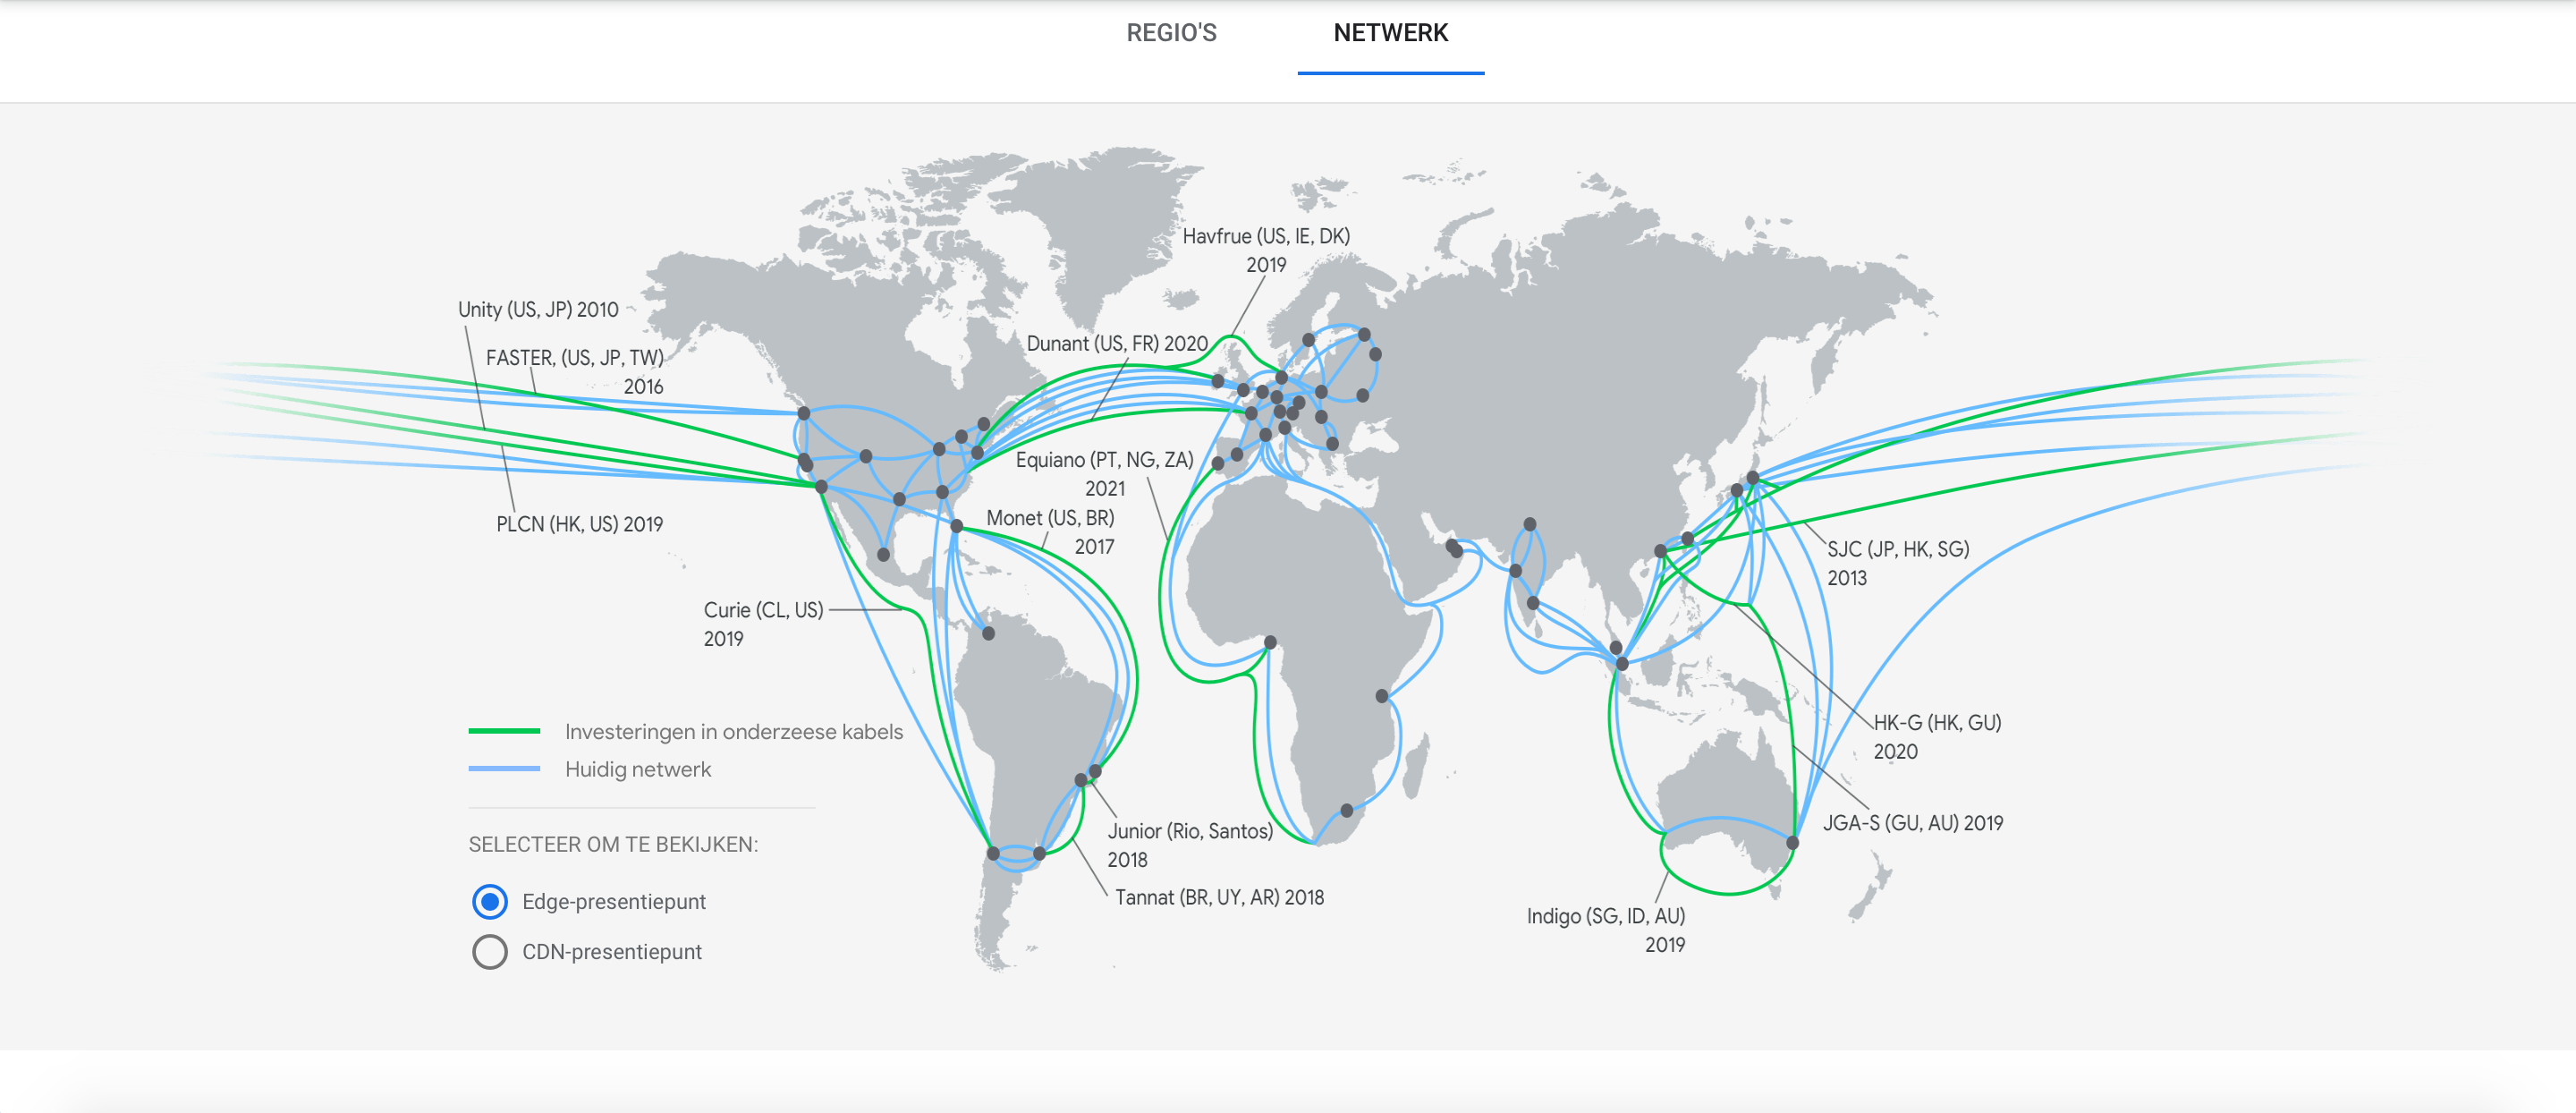
\includegraphics[width=\linewidth]{/Users/kenzie/Documents/HoGent/Bachelorproef/Images/GCP_NetwerkKaart.png}
    \caption{Figuur van \href{}{Google Cloud website}. Figuur toont de connectiviteit van de verschillende datacenters verspreid over de wereld.}
    \label{fig:GCP_NetwerkKaart}
\end{figure}

\section{Proof Of Concept}
\subsection{Beschrijving}
Omdat Aucxis met een Microsoft georiënteerde werkwijze zit, moet er worden aangetoond dat dit mogelijk is om te realiseren met GCP. Voor deze Proof Of Concept (POC) wordt er een CI/CD pijpleiding geconfigureerd. Hierin wordt er een simpele .NET Core applicatie gecompileerd en getest. Deze zal dan zodanig verpakt worden dat het op een fileserver buiten de Cloud, dus lokaal op eigen servers, gebruikt kan worden in een test omgeving.

Er wordt allereerst een GitHub aangemaakt waarin een simpel voorbeeld .Net applicatie geplaatst zal worden. Hier wordt dan naast de te gebruiken Docker container ook een YML-file gedefinieerd waarin staat welke compilatie stappen er allemaal zullen moeten gebeuren. Hierna wordt de daadwerkelijke pijpleiding gemaakt op GCP waarin de link wordt gemaakt naar de GitHub repository. Deze pijpleiding wordt dan gestart en getest waarna de bevindingen genoteerd zijn.

\subsection{Moeilijkheden}
\subsection{Uitvoering}
\subsection{Resultaat \& Bedenkingen}
\section{Vergelijking met Azure DeVops}
\subsection{Beschrijving}
\subsection{Uitvoering}
\subsection{Resultaat \& Bedenkingen}

%Aantal woorden: 3933%